% Cross-source audit of the FireSET California fire list, run of 2026-10-13.
% Build: latexmk -pdf findings.tex   (TeX Live with tikz, pgfplots, booktabs)
\documentclass[11pt,a4paper]{article}

\usepackage[margin=2.3cm]{geometry}
\usepackage[T1]{fontenc}
\usepackage[utf8]{inputenc}
\usepackage{lmodern}
\usepackage{microtype}
\usepackage{booktabs}
\usepackage{array}
\usepackage{multirow}
\usepackage{xcolor}
\usepackage{graphicx}
\usepackage{adjustbox}
\usepackage{tabularx}
\usepackage{caption}
\usepackage{enumitem}
\usepackage{amsmath}
\usepackage{tikz}
\usetikzlibrary{arrows.meta,positioning,shapes.geometric,fit,calc,backgrounds}
\usepackage{pgfplots}
\pgfplotsset{compat=1.18}
\usepackage[colorlinks=true,linkcolor=blue!60!black,urlcolor=blue!60!black,citecolor=blue!60!black]{hyperref}

\definecolor{irwin}{HTML}{2A78D6}
\definecolor{calfire}{HTML}{D6552A}
\definecolor{usfs}{HTML}{2E8B57}
\definecolor{mtbs}{HTML}{8E44AD}
\definecolor{sat}{HTML}{B8860B}
\definecolor{fireset}{HTML}{333333}
\definecolor{grey}{HTML}{6E6E6E}
\definecolor{paleblue}{HTML}{E8F0FB}
\definecolor{paleorange}{HTML}{FBECE4}
\definecolor{palegreen}{HTML}{E6F3EA}

\tikzset{
  box/.style={draw, rounded corners=2pt, align=center, font=\small, minimum height=8mm, inner sep=4pt},
  stage/.style={box, fill=paleblue, minimum width=24mm},
  data/.style={box, fill=palegreen, minimum width=24mm},
  src/.style={box, fill=white, minimum width=22mm},
  dec/.style={diamond, draw, aspect=2.2, align=center, font=\small, inner sep=1pt, fill=paleorange},
  flow/.style={-{Latex[length=2.5mm]}, thick},
  copy/.style={-{Latex[length=2.2mm]}, thick, irwin},
  lbl/.style={font=\scriptsize, fill=white, inner sep=1pt},
}

\captionsetup{font=small, labelfont=bf}
\newcolumntype{L}[1]{>{\raggedright\arraybackslash}p{#1}}
\newcolumntype{Y}{>{\raggedright\arraybackslash}X}
% every diagram is scaled down only if it would exceed the text width
\newenvironment{fitfig}{\begin{adjustbox}{max width=\textwidth,center}}{\end{adjustbox}}
\setlist{nosep}

\title{\textbf{Where Does FireSET's Fire Data Come From?}\\[4pt]
\large A cross-source audit of ignition points, perimeters, timing, size and cause\\
for 586 California wildfires, 2018--2025}
\author{fire-data-revalidate \\ \small\url{https://github.com/utkrshkmr/fire-data-revalid}}
\date{Run of 13 October 2026}

\begin{document}
\maketitle

\begin{abstract}
\noindent FireSET is a 586-fire California training set whose locations and times are taken from NIFC's WFIGS
(IRWIN) feed and whose perimeters come from CAL~FIRE FRAP. We asked how far those values can be corroborated
by every other U.S. federal and California agency source that reports the same fires, and by three satellite
products. We built and ran \texttt{fire-source-audit} (\texttt{fsa}), a probe\,$\to$\,fetch\,$\to$\,match\,$\to$\,consensus
pipeline over 13 agency sources and 3 satellite products. Three results stand out. (1)~\emph{The sources are
far less independent than their catalog suggests}: FPA-FOD, InFORM, FireStat and MTBS largely re-publish the
IRWIN record, so for a third of the fires there is no second agency location at all. (2)~\emph{Where independent
points exist they disagree by about 800\,m}, and by more than 2\,km on one fire in six. FireSET's point is within
100\,m of the best-supported agency point on 435 fires; 62 fires have a point that lies outside the final
perimeter while another agency point lies inside it. (3)~\emph{Discovery times carry systematic clock errors}:
USFS FireStat runs 2\,h ahead of Pacific time in 2018--19, and the USFS web service re-labels those values as
UTC, producing $-5$\,h and $-7$\,h offsets that propagate into InFORM and FPA-FOD. GOES-R's first detection falls a
median 10 minutes after FireSET's start time, which independently confirms FireSET's timing. Seven defects in the
source catalog had to be fixed before any of these conclusions could be drawn; they are documented so the audit
can be re-run.
\end{abstract}

\tableofcontents
\clearpage

%======================================================================
\section{Question and scope}

FireSET (\emph{VIIRS-Qualified California Wildfires, 2018--2025}, finalised 2026-08-30) holds one row per fire
for 586 fires: 538 individual fires and 48 components of complexes. Its \texttt{Ignition\_Lat/Lon} are IRWIN
incident points obtained through NIFC WFIGS, \texttt{Start\_Local} is IRWIN's discovery time
(\texttt{FireDiscoveryDateTime}), and the perimeter and \texttt{GIS\_ACRES} come from CAL~FIRE FRAP. The dataset documentation states that no row
has been hand-edited.

The brief for this audit was to \emph{corroborate and understand} those values against every other
government source that reports them: where did each fire start, what was its final perimeter, when was it
discovered and contained, how big was it, and what caused it. A secondary question was raised explicitly: are
FPA-FOD, CAL~FIRE and IRWIN really independent of one another, or do they copy each other?

\paragraph{What counts as a source.} Only records published by a U.S.\ federal agency or the State of
California, plus physical satellite measurements from NASA and NOAA. Academic compilations (ICS-209-PLUS),
commercial feeds and community mirrors were excluded by design. Table~\ref{tab:sources} lists what was used.

\begin{table}[h]
\centering\footnotesize
\caption{Sources used in the run. ``Lineage'' is the upstream system whose record the source carries; sources
with the same lineage are counted once in any consensus. Tier A = record of the responsible agency or an
independent physical measurement; B = official but operational or second-hand; C = derivative merge.}
\label{tab:sources}
\begin{tabularx}{\textwidth}{@{}L{3.2cm}L{2.3cm}YL{2.7cm}c@{}}
\toprule
Source & Agency & Gives & Lineage & Tier\\
\midrule
WFIGS Incident Locations & NIFC / IRWIN & point, times, size, cause & IRWIN & A\\
InFORM Fire Occurrence (public) & NIFC & final-report point, times, size, cause & per record$^\dagger$ & A\\
CAL FIRE incident list & CAL FIRE & map point, start time, acres & CALFIRE-OPS & A\\
USFS EDW FireStat points & USDA Forest Service & point, times, size, cause & USFS-FIRESTAT & A\\
FPA-FOD 7th ed.\ (1992--2024) & USFS Research & point, date+time, size, cause & per record$^\dagger$ & A\\
MTBS fire-occurrence points & USGS / USFS GTAC & reported point (in \texttt{Event\_ID}), date, acres & MTBS-REPORTED & B\\
\addlinespace
CAL FIRE FRAP perimeters & CAL FIRE & final perimeter, dates, acres, cause & CALFIRE-FRAP & A\\
NIFC perimeter history (to 2021) & NIFC & perimeter, acres & from \texttt{SOURCE} & A\\
WFIGS Interagency Perimeters & NIFC & latest perimeter, acres & NIFC-WFIGS & A\\
USFS EDW final perimeters & USDA Forest Service & perimeter, acres & USFS-FIRESTAT & A\\
MTBS burned-area boundaries & USGS / USFS GTAC & Landsat dNBR perimeter, acres & MTBS & A\\
USGS combined fire polygons & USGS & merged perimeter (to 2020) & USGS-COMBINED & C\\
\addlinespace
NASA FIRMS VIIRS 375\,m & NASA & active-fire detections (S-NPP, NOAA-20) & SAT-LEO & A\\
NOAA GOES-R ABI FDC & NOAA & 5-minute fire detections, 2\,km & SAT-GEO & A\\
NOAA HMS fire points & NOAA NESDIS & analyst-checked daily points & SAT-HMS & B\\
\bottomrule
\multicolumn{5}{@{}l@{}}{$^\dagger$Compiled sources take the lineage of the system each record was copied from (\S\ref{sec:independence}).}
\end{tabularx}
\end{table}

%======================================================================
\section{Method}

\subsection{Pipeline}

Figure~\ref{fig:pipeline} shows the five stages. Every stage is resumable and every raw pull is cached, so the
analysis can be re-run offline. The full 586-fire run takes about 100 seconds on 16 cores once the cache is
populated; fetching takes 15--30 minutes of polite (0.3\,s-spaced) requests plus about 20 minutes for the optional
GOES-R scan.

\begin{figure}[h]
\begin{fitfig}
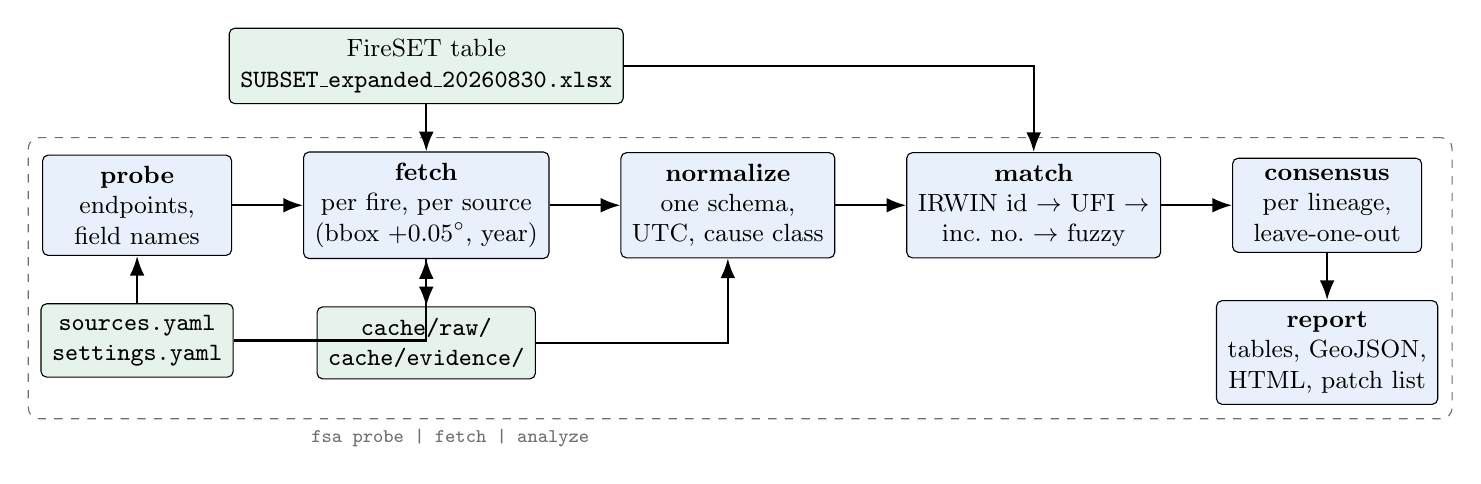
\begin{tikzpicture}[node distance=6mm and 9mm]
  \node[stage] (probe) {\textbf{probe}\\endpoints,\\field names};
  \node[stage, right=of probe] (fetch) {\textbf{fetch}\\per fire, per source\\(bbox $+0.05^\circ$, year)};
  \node[stage, right=of fetch] (norm) {\textbf{normalize}\\one schema,\\UTC, cause class};
  \node[stage, right=of norm] (match) {\textbf{match}\\IRWIN id $\to$ UFI $\to$\\inc.\ no.\ $\to$ fuzzy};
  \node[stage, right=of match] (cons) {\textbf{consensus}\\per lineage,\\leave-one-out};
  \node[stage, below=of cons] (rep) {\textbf{report}\\tables, GeoJSON,\\HTML, patch list};
  \node[data, below=of fetch] (cache) {\texttt{cache/raw/}\\\texttt{cache/evidence/}};
  \node[data, below=of probe] (cfg) {\texttt{sources.yaml}\\\texttt{settings.yaml}};
  \node[data, above=of fetch] (xlsx) {FireSET table\\\texttt{SUBSET\_expanded\_20260830.xlsx}};
  \draw[flow] (probe) -- (fetch);
  \draw[flow] (fetch) -- (norm);
  \draw[flow] (norm) -- (match);
  \draw[flow] (match) -- (cons);
  \draw[flow] (cons) -- (rep);
  \draw[flow] (fetch) -- (cache);
  \draw[flow] (cache) -| (norm);
  \draw[flow] (cfg) -- (probe);
  \draw[flow] (cfg) -| (fetch);
  \draw[flow] (xlsx) -- (fetch);
  \draw[flow] (xlsx.east) -| (match.north);
  \begin{scope}[on background layer]
    \node[fit=(probe)(fetch)(norm)(match)(cons)(rep), draw=grey, dashed, rounded corners, inner sep=5pt,
          label={[grey,font=\scriptsize]below left:\texttt{fsa probe | fetch | analyze}}] {};
  \end{scope}
\end{tikzpicture}
\end{fitfig}
\caption{The \texttt{fsa} pipeline. Fetch runs where the agency hosts are reachable (a login node); match,
consensus and report run anywhere from the cache.}
\label{fig:pipeline}
\end{figure}

\subsection{Matching}

For each fire, candidate records within the FireSET bounding box (buffered $0.05^\circ$) and the fire's season
are scored. Identifier evidence wins outright: the same IRWIN GUID scores 1.00, the same
\texttt{UniqueFireIdentifier} 0.97, the same incident number in the same year with a consistent location 0.90.
Otherwise a fuzzy score combines name similarity (0.45), date proximity (0.25), place (0.20) and size (0.10),
capped at 0.89 and halved when the names differ. A record is accepted at 0.60, and flagged ambiguous when a
different record is within 0.05 of it. Two guards were added during the run: a fuzzy match more than 15 days
from the FireSET start, or a perimeter dated before the fire or over a year after it, is rejected as another
fire with the same name (21 such matches existed before the guard, e.g.\ CAL~FIRE's ``Peak Fire'' of 2024 for
Peak 2023).

\subsection{Lineages and copy detection}
\label{sec:method-lineage}

Sources that re-publish one upstream record must not be allowed to ``agree'' with each other. The catalog
assigns each source a lineage, but the run showed that is not enough (\S\ref{sec:independence}), so two
mechanisms were added. First, compiled sources take their lineage \emph{per record}: FPA-FOD from its
\texttt{SOURCE\_SYSTEM} column, InFORM from \texttt{CreatedBySystem}. Second, for each fire, two reported points
from different lineages are treated as one report when they are within 5\,m (float32 storage and Web Mercator
round trips move a copied point by 1--2\,m), or when one is exactly the other rounded to three or four decimals
(the MTBS \texttt{Event\_ID} encodes thousandths of a degree). Their lineages are merged for that fire before any
consensus is built. Every detected copy is written to \texttt{identical\_point\_pairs.csv}.

\subsection{Consensus and per-source error}

The ignition consensus is the trust-weighted geometric median (Weiszfeld) of one medoid point per lineage. The
agreement class is set by the largest distance between any two lineages: \emph{agree} $\le 500$\,m,
\emph{minor} $\le 2$\,km, \emph{major} beyond, or \emph{single lineage}. The perimeter consensus rasterises one
polygon per lineage at 30\,m and keeps cells covered by at least half the lineages (with two lineages, their
union). Every per-source error compares the source with the consensus of the \emph{other} lineages, so a
source never grades itself; with only two lineages that disagree by more than 2\,km, no reference is formed.

\subsection{Satellite evidence}

VIIRS detections inside the consensus perimeter ($+1$\,km) give the first-overpass time and centre; detections
more than 12\,h before the earliest reported discovery are ignored, since they are almost always a neighbouring
or earlier fire. GOES-R ABI fire-detection files (every 5 minutes) are scanned from 6\,h before to 3\,h after
the reported discovery within 5\,km of the FireSET point; the earliest fire-mask pixel is the tightest
independent bound on ignition time. NOAA HMS analyst points are kept apart from VIIRS because they mix coarse
GOES and AVHRR pixels with analyst timing.

Whole-hour offsets of 2, 5, 7 or 8\,h between a source's discovery time and the other lineages are suspected
clock or time-zone errors. Both sides of such a pair look offset, so the satellite's first heat (GOES, else HMS,
else VIIRS) acts as referee: the side farther from it is flagged.

%======================================================================
\section{The catalog had to be corrected first}
\label{sec:catalog}

The delivered source catalog had been checked against live service \emph{metadata}; the run checked it against
live \emph{data}. Seven defects would each have produced false disagreements. Table~\ref{tab:fixes} lists them;
all are fixed in \texttt{config/sources.yaml} and the adapters, with regression tests.

\begin{table}[h]
\centering\small
\caption{Defects found by running against live data, and what the audit would have reported without the fix.}
\label{tab:fixes}
\begin{tabular}{@{}L{2.6cm}L{8.1cm}L{4.4cm}@{}}
\toprule
Source & Problem & Effect if left alone\\
\midrule
WFIGS (IRWIN) & The config compared \texttt{InitialLatitude/Longitude}. FireSET uses the feature geometry (IRWIN's
\emph{current} point of origin): it matches the geometry on 478 of 479 fires. The first-report point differs
from it by $>500$\,m on 193 fires and by $>5$\,km on 56. & FireSET ``disagrees'' with its own source on a third
of fires.\\
\addlinespace
InFORM & No \texttt{IrwinID} or text cause fields; IDs are in \texttt{RelatedIrwinIDs}, cause is an integer
\texttt{FireCauseID}. \texttt{FinalAcres} is null for every California record. California 2018--19 records are
FireStat/WFMI back-fill, not IRWIN. & No ID matches, no cause, no size; wrong lineage.\\
\addlinespace
CAL FIRE incidents & API moved to \texttt{incidents.fire.ca.gov} (old host returns HTTP~403 to non-generic user
agents); needs \texttt{\&year=} or only the current season is returned; \texttt{Started} is UTC, not Pacific; 294
records carry a bulk ``extinguished'' date of 2019-01-04. & Source unreachable.\\
\addlinespace
FPA-FOD 7th ed. & No \texttt{IRWIN\_ID} or \texttt{UNIQUE\_FIRE\_ID} columns. Records are copies of other systems
(\texttt{SOURCE\_SYSTEM}): 2020 = IA-IRWIN, 2021--24 = IA-INFORM. & Counted as independent of FireSET when it is the
same IRWIN record.\\
\addlinespace
MTBS points & \texttt{BurnBndLat/Lon} is the burned-area centroid (Camp 2018: 10\,km from the origin). The reported
origin is encoded in \texttt{Event\_ID}. & Every large fire a ``major disagreement''.\\
\addlinespace
FRAP, FPA-FOD, MTBS dates & Calendar dates stored as 00:00 UTC were shifted into the previous Pacific day. &
Every alarm date one day early.\\
\addlinespace
CAL FIRE FIRIS view & Holds only the current season (476 polygons, 2026). & False same-name matches; now
disabled.\\
\bottomrule
\end{tabular}
\end{table}

Two engineering problems also surfaced only at full scale. Raster-traced perimeters (MTBS, FIRIS) carry tens
of thousands of vertices, and the exact boundary Hausdorff distance is $O(nm)$: the Dixie Fire alone took
222\,s, and buffering its perimeter for the detection zone took a further minute. Simplifying boundaries to
10\,m (or $\sqrt{\text{area}}/500$ for very large fires) before the distance, and buffering a simplified polygon,
brought Dixie to 36\,s; running fires in parallel processes brought the whole run to 100\,s. Separately, 21 GOES
files carried time units that xarray refuses to decode; the scan now reads them with \texttt{decode\_times=False},
since the timestamp is in the file name.

%======================================================================
\section{How independent are the sources?}
\label{sec:independence}

\subsection{Points}

The brief asked whether FPA-FOD, CAL~FIRE and IRWIN are independent. The answer is that \emph{most of the
catalog is one record seen through several windows}. Figure~\ref{fig:copies} shows the copy relationships
detected per fire by the rule of \S\ref{sec:method-lineage}; Table~\ref{tab:lineage} shows what the compiled
sources actually contain.

\begin{figure}[h]
\begin{fitfig}
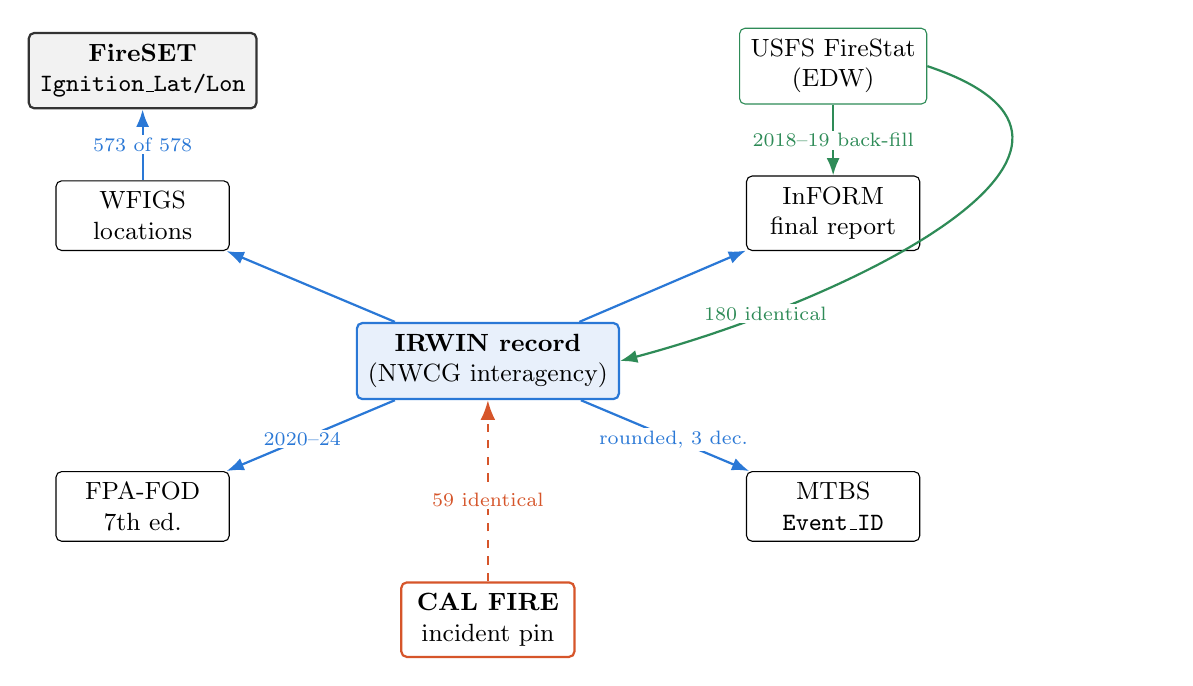
\begin{tikzpicture}[node distance=9mm and 16mm]
  \node[src, fill=paleblue, draw=irwin, thick, minimum width=32mm] (irwin) {\textbf{IRWIN record}\\(NWCG interagency)};
  \node[src, above left=of irwin] (wfigs) {WFIGS\\locations};
  \node[src, above right=of irwin] (inform) {InFORM\\final report};
  \node[src, below left=of irwin] (fpa) {FPA-FOD\\7th ed.};
  \node[src, below right=of irwin] (mtbs) {MTBS\\\texttt{Event\_ID}};
  \node[src, above=of wfigs, fill=black!5, draw=fireset, thick] (fs) {\textbf{FireSET}\\\texttt{Ignition\_Lat/Lon}};
  \node[src, above=of inform, draw=usfs] (firestat) {USFS FireStat\\(EDW)};
  \node[src, below=of irwin, draw=calfire, thick, yshift=-14mm] (cf) {\textbf{CAL FIRE}\\incident pin};
  \draw[copy] (irwin) -- (wfigs);
  \draw[copy] (irwin) -- (inform);
  \draw[copy] (irwin) -- node[lbl, pos=.55]{2020--24} (fpa);
  \draw[copy] (irwin) -- node[lbl, pos=.55]{rounded, 3 dec.} (mtbs);
  \draw[copy] (wfigs) -- node[lbl]{573 of 578} (fs);
  \draw[copy, usfs] (firestat) -- node[lbl]{2018--19 back-fill} (inform);
  \draw[copy, usfs] (firestat.east) .. controls +(30mm,-10mm) and +(30mm,8mm) .. node[lbl, pos=.8]{180 identical} (irwin.east);
  \draw[flow, calfire, dashed] (cf) -- node[lbl, pos=.45]{59 identical} (irwin);
\end{tikzpicture}
\end{fitfig}
\caption{Who copies whom. Solid blue and green arrows: the same point re-published (within 5\,m, or a
3--4-decimal rounding); the dashed arrow: an independent record that nevertheless carries the same coordinates
on some fires. Counts are fires among the 586 where the two points are identical. FireSET's ignition point is
IRWIN's current point on 573 fires; InFORM, FPA-FOD (from 2020) and the MTBS \texttt{Event\_ID} carry the same
point; FireStat equals IRWIN on 180 fires. Only the CAL~FIRE incident pin is routinely a separate observation.}
\label{fig:copies}
\end{figure}

\begin{table}[h]
\centering\footnotesize
\caption{What the compiled sources actually contain for the 586 fires, by the system each record was copied from.}
\label{tab:lineage}
\begin{tabular}{@{}llr@{\quad}llr@{}}
\toprule
\multicolumn{3}{@{}l}{FPA-FOD 7th ed.\ (459 matched fires)} & \multicolumn{3}{l@{}}{InFORM public (545 matched fires)}\\
\cmidrule(r){1-3}\cmidrule(l){4-6}
\texttt{SOURCE\_SYSTEM} & lineage & fires & \texttt{CreatedBySystem} & lineage & fires\\
\midrule
IA-IRWIN, IA-INFORM & IRWIN & 340 & CAD systems via IRWIN & IRWIN & 458\\
FS-FIRESTAT & USFS-FIRESTAT & 56 & FireStat & USFS-FIRESTAT & 53\\
DOI-WFMI & DOI-WFMI & 35 & WFMI & DOI-WFMI & 34\\
IA-ICS209 & ICS209 & 14 & & &\\
ST-NASF, ST-CACDF & CALFIRE-STATE & 10 & & &\\
FWS-FMIS, IA-MTBS & other & 4 & & &\\
\bottomrule
\end{tabular}
\end{table}

After merging copies, the number of \emph{independent} reporting lineages per fire is small
(Table~\ref{tab:nlineages}): four fires have no agency point, 195 have exactly one (almost always IRWIN), and
only 52 have three or more. Where a second lineage exists it is usually the CAL~FIRE incident pin, or a
FireStat or state record from 2018--19 before those systems were folded into IRWIN. FPA-FOD remains valuable
for 2018--19, when its records are FireStat, WFMI and state copies that predate IRWIN, but for 2020 onward it
cannot confirm FireSET.

\begin{table}[h]
\centering\small
\caption{Independent reporting lineages per fire, after merging copied points.}
\label{tab:nlineages}
\begin{tabular}{@{}lrrrrr@{}}
\toprule
Lineages & 0 & 1 & 2 & 3 & 4\\
\midrule
Fires & 4 & 195 & 335 & 49 & 3\\
\bottomrule
\end{tabular}
\end{table}

\subsection{Perimeters}

Perimeters behave the same way (Figure~\ref{fig:perims}). FRAP, WFIGS, USFS EDW and the NIFC history layer
share one polygon on most fires: the intersection-over-union is at least 0.999 on 69--94\% of the fires they
have in common. MTBS, mapped from Landsat differenced burn ratios rather than by incident teams, is the only
independent perimeter. It agrees with the agency polygon at a median IoU of 0.94 and is a median 2\%
\emph{larger}, not smaller as the catalog expected (``unburned islands are excluded''); unburned islands
inside agency polygons are evidently outweighed by burned area outside them.

\begin{figure}[h]
\begin{fitfig}
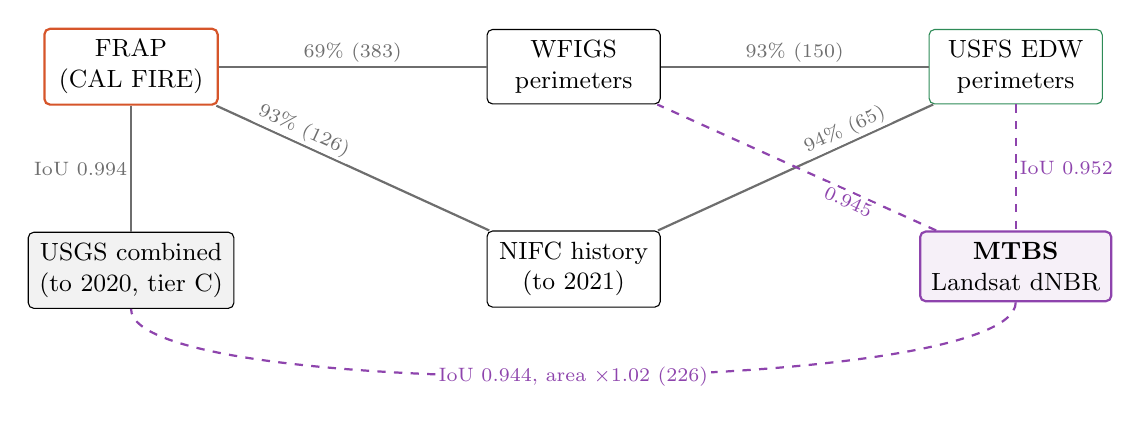
\begin{tikzpicture}[node distance=16mm and 34mm]
  \node[src, draw=calfire, thick] (frap) {FRAP\\(CAL FIRE)};
  \node[src, right=of frap] (wf) {WFIGS\\perimeters};
  \node[src, right=of wf, draw=usfs] (edw) {USFS EDW\\perimeters};
  \node[src, below=of frap, fill=black!5] (usgs) {USGS combined\\(to 2020, tier C)};
  \node[src, below=of wf] (ifph) {NIFC history\\(to 2021)};
  \node[src, below=of edw, draw=mtbs, thick, fill=mtbs!8] (mtbs) {\textbf{MTBS}\\Landsat dNBR};
  \draw[thick, grey] (frap) -- node[lbl, above]{69\% (383)} (wf);
  \draw[thick, grey] (wf) -- node[lbl, above]{93\% (150)} (edw);
  \draw[thick, grey] (frap) -- node[lbl, sloped, above, pos=.3]{93\% (126)} (ifph);
  \draw[thick, grey] (edw) -- node[lbl, sloped, above, pos=.3]{94\% (65)} (ifph);
  \draw[thick, grey] (frap) -- node[lbl, left]{IoU 0.994} (usgs);
  \draw[thick, mtbs, dashed] (edw) -- node[lbl, right]{IoU 0.952} (mtbs);
  \draw[thick, mtbs, dashed] (mtbs) -- node[lbl, sloped, below, pos=.3]{0.945} (wf);
  \draw[thick, mtbs, dashed] (mtbs.south) .. controls +(0,-12mm) and +(0,-12mm) .. node[lbl, pos=.5]{IoU 0.944, area $\times$1.02 (226)} (usgs.south);
\end{tikzpicture}
\end{fitfig}
\caption{Perimeter agreement between sources. Grey edges: effectively the same polygon passed between systems;
the label is the share of shared fires with IoU $\ge 0.999$ (number of shared fires in brackets), or the median
IoU. Dashed purple edges: MTBS, the one independently mapped perimeter, with its median IoU against each agency
layer.}
\label{fig:perims}
\end{figure}

%======================================================================
\section{Ignition points}

\subsection{Agreement across independent lineages}

\begin{figure}[h]
\centering
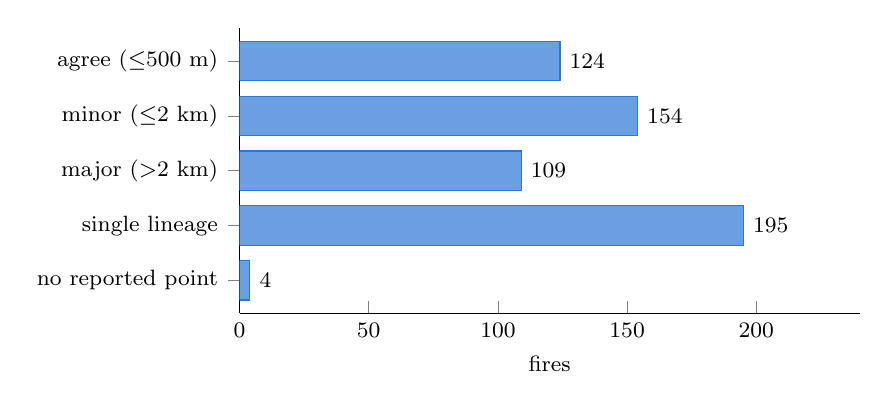
\begin{tikzpicture}
\begin{axis}[
  xbar, bar width=5mm, width=0.78\textwidth, height=5.2cm,
  xlabel={fires}, xmin=0, xmax=240,
  ytick={1,2,3,4,5}, yticklabels={{no reported point},{single lineage},{major ($>$2 km)},{minor ($\le$2 km)},{agree ($\le$500 m)}},
  ymin=0.4, ymax=5.6, nodes near coords, nodes near coords align={horizontal},
  every node near coord/.append style={font=\footnotesize},
  axis x line*=bottom, axis y line*=left, tick label style={font=\footnotesize}, label style={font=\footnotesize},
]
\addplot[fill=irwin!70, draw=irwin] coordinates {(124,5) (154,4) (109,3) (195,2) (4,1)};
\end{axis}
\end{tikzpicture}
\caption{Ignition agreement across independent lineages, 586 fires. ``Agree'' means every independent agency
point lies within 500\,m of every other.}
\label{fig:agree}
\end{figure}

Among the 387 fires with two or more independent lineages, 124 agree within 500\,m, 154 differ by up to 2\,km
and 109 differ by more than 2\,km (Figure~\ref{fig:agree}). Table~\ref{tab:ignerr} grades each source against
the consensus of the \emph{other} lineages. The sources are remarkably alike: a median disagreement of
700--900\,m and a 90th percentile of 4--5\,km, whichever agency is doing the reporting. MTBS's
\texttt{Event\_ID} point is coarser (1.3\,km median), as expected for a 3-decimal encoding of a point that is
itself a copy. About 5\% of WFIGS points carry only two decimals, i.e.\ roughly $\pm$550\,m of precision.
Roughly a quarter of agency points sit more than 375\,m outside the final perimeter, which for a point of
origin is implausible, and a sign that many ``ignition'' points are dispatch or report locations.

\begin{table}[h]
\centering\small
\caption{Distance from each source's ignition point to the consensus of the other independent lineages
(leave-one-lineage-out). ``Outside'' = more than 375\,m outside the consensus perimeter.}
\label{tab:ignerr}
\begin{tabular}{@{}lrrrrrr@{}}
\toprule
Source & $n$ & median & 90th pct & $>2$\,km & outside & median to first VIIRS\\
\midrule
USFS FireStat (EDW) & 139 & 719\,m & 4.0\,km & 13\% & 9\% & 634\,m\\
InFORM & 348 & 748\,m & 4.6\,km & 15\% & 17\% & 790\,m\\
WFIGS / IRWIN & 363 & 793\,m & 4.6\,km & 16\% & 23\% & 862\,m\\
CAL FIRE incidents & 340 & 805\,m & 5.0\,km & 21\% & 28\% & 1.20\,km\\
FPA-FOD & 280 & 907\,m & 4.8\,km & 17\% & 18\% & 793\,m\\
MTBS (\texttt{Event\_ID}) & 143 & 1.33\,km & 5.7\,km & 25\% & 22\% & 1.40\,km\\
\midrule
FireSET (vs all lineages) & 578 & 152\,m & 1.9\,km & 10\% & 24\% & 873\,m\\
\bottomrule
\end{tabular}
\end{table}

\subsection{The first-report point is not the point of origin}

IRWIN keeps two locations per incident: \texttt{InitialLatitude/Longitude}, entered at first report, and the
feature geometry, which is updated as the incident is investigated. They differ by more than 500\,m on 193 of
478 fires and by more than 5\,km on 56. FireSET correctly uses the current point. Any future comparison that
uses the \texttt{Initial*} fields (as the delivered catalog did) measures the evolution of IRWIN's own record,
not disagreement between agencies.

\subsection{FireSET corrections}
\label{sec:patch}

FireSET's point lies within 100\,m of the best-supported agency point on 435 fires and within 500\,m on 459
(Figure~\ref{fig:delta}). The remaining 127 fires are listed in \texttt{fireset\_ignition\_patch.csv}
with old and new coordinates, the source and confidence of the new point, both points' signed distance to the
consensus perimeter and to the first VIIRS overpass, and an \emph{action} decided by the rule in
Figure~\ref{fig:decision}.

\begin{figure}[h]
\centering
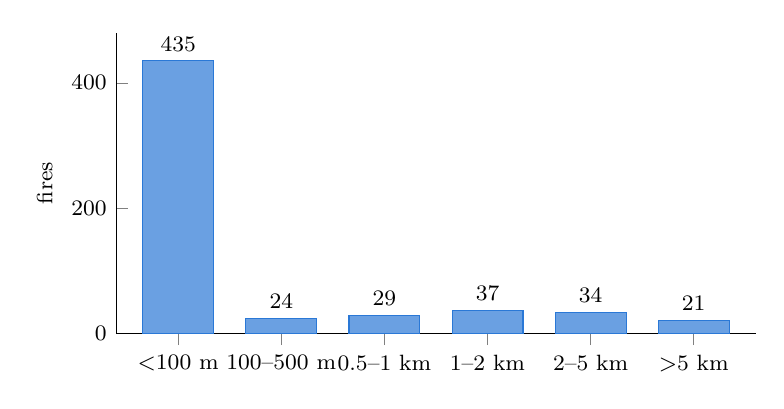
\begin{tikzpicture}
\begin{axis}[
  ybar, bar width=9mm, width=0.8\textwidth, height=5.4cm,
  ylabel={fires}, ymin=0, ymax=480,
  xtick={1,...,6}, xticklabels={{$<$100 m},{100--500 m},{0.5--1 km},{1--2 km},{2--5 km},{$>$5 km}},
  xmin=0.4, xmax=6.6, nodes near coords, every node near coord/.append style={font=\footnotesize},
  axis x line*=bottom, axis y line*=left, tick label style={font=\footnotesize}, label style={font=\footnotesize},
]
\addplot[fill=irwin!70, draw=irwin] coordinates {(1,435) (2,24) (3,29) (4,37) (5,34) (6,21)};
\end{axis}
\end{tikzpicture}
\caption{Distance from FireSET's current \texttt{Ignition\_Lat/Lon} to the recommended agency point, 580 fires
with a FireSET point.}
\label{fig:delta}
\end{figure}

\begin{figure}[h]
\begin{fitfig}
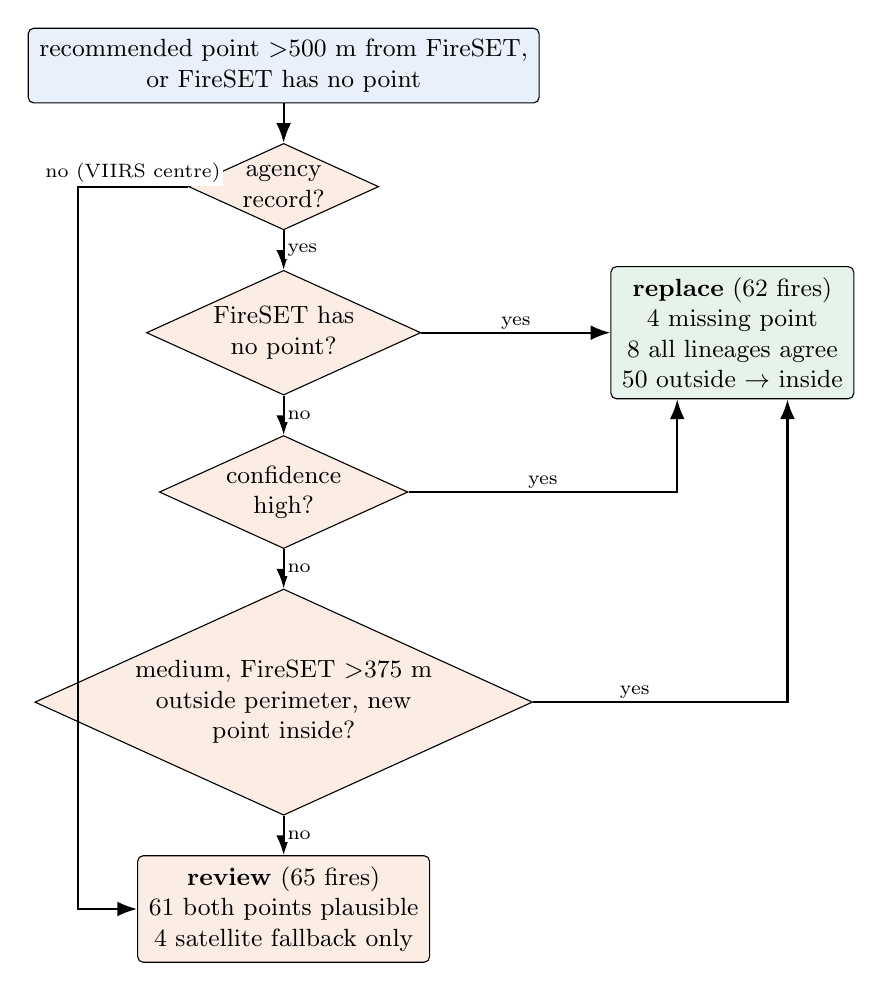
\begin{tikzpicture}[node distance=5mm and 10mm, every node/.style={font=\small}]
  \node[box, fill=paleblue] (start) {recommended point $>$500 m from FireSET,\\or FireSET has no point};
  \node[dec, below=of start] (d1) {agency\\record?};
  \node[dec, below=of d1] (d2) {FireSET has\\no point?};
  \node[dec, below=of d2] (d3) {confidence\\high?};
  \node[dec, below=of d3] (d4) {medium, FireSET $>$375 m\\outside perimeter, new\\point inside?};
  \node[box, fill=palegreen, right=of d2, xshift=14mm] (rep) {\textbf{replace} (62 fires)\\4 missing point\\8 all lineages agree\\50 outside $\to$ inside};
  \node[box, fill=paleorange, below=of d4] (rev) {\textbf{review} (65 fires)\\61 both points plausible\\4 satellite fallback only};
  \draw[flow] (start) -- (d1);
  \draw[flow] (d1) -- node[lbl, right]{yes} (d2);
  \draw[flow] (d2) -- node[lbl, right]{no} (d3);
  \draw[flow] (d3) -- node[lbl, right]{no} (d4);
  \draw[flow] (d4) -- node[lbl, right]{no} (rev);
  \draw[flow] (d2) -- node[lbl, above]{yes} (rep);
  \draw[flow] (d3.east) -| node[lbl, above, pos=.25]{yes} ([xshift=-7mm]rep.south);
  \draw[flow] (d4.east) -| node[lbl, above, pos=.2]{yes} ([xshift=7mm]rep.south);
  \draw[flow] (d1.west) -- node[lbl, above]{no (VIIRS centre)} ++(-14mm,0) |- (rev.west);
\end{tikzpicture}
\end{fitfig}
\caption{How each proposed correction is classified. ``Confidence'' is high when all reporting lineages agree,
medium when one lineage reports or the winner is strongly supported, low otherwise.}
\label{fig:decision}
\end{figure}

\paragraph{Replace (62 fires).} Fifty are cases where FireSET's point lies outside the final perimeter while a
second agency point lies inside it; eight are cases where every independent lineage agrees on a point FireSET
does not carry; four fill a missing point. The median move is 1.5\,km. The replacement points come from the
CAL~FIRE incident list (31), InFORM final reports (25) and FPA-FOD (6). Two examples:

\begin{itemize}
\item \textbf{Sites 2024.} FireSET's point is 6.4\,km outside the 19,115-acre perimeter. InFORM's final report
for the \emph{same} IRWIN incident, and the CAL~FIRE pin, agree on a point inside the perimeter 1.1--1.25\,km
from the first VIIRS overpass. IRWIN's own first-report location is 11\,km from its current one: the record
was moved once and FireSET captured the wrong state.
\item \textbf{O'Neals 2018.} FireSET carries a two-decimal point 7.7\,km from the 433-acre perimeter. CAL~FIRE's
pin and the state (ST-NASF) record in FPA-FOD agree within 17\,m, 800\,m from the perimeter.
\end{itemize}

\paragraph{Review (65 fires).} Both points are plausible (often both inside the perimeter), or the only
alternative is the centre of the first VIIRS overpass (4 fires, including 5-6 Cascade Creek 2020, whose FireSET
point is 30\,km from its 260-acre perimeter and for which no agency record matched at all).

\paragraph{Caveat.} Thirty-one replacements rest on the CAL~FIRE incident pin. That pin is a map location for
the public, not an investigated origin, so rows where it is the only support deserve a look before they are
applied. The scoring also favours points inside the final perimeter, which is right for an origin but is not
proof of one.

%======================================================================
\section{Discovery times}

\subsection{Agreement and satellite confirmation}

IRWIN, CAL~FIRE and the state records agree on discovery time: median offset zero, 60--64\% within 15 minutes.
GOES-R's first fire-mask detection within 5\,km of the FireSET point lands a median 0.17\,h (10 minutes) after
the reported discovery, and within one hour on 275 of the 391 fires where it found anything
(Table~\ref{tab:sat}). This is the strongest independent confirmation in the audit: FireSET's
\texttt{Start\_Local} is a genuine report time, not a date-only or back-filled value.

\begin{table}[h]
\centering\small
\caption{Satellite first detection minus reported discovery, hours. VIIRS: first detection inside the
perimeter within the lead window; GOES: first fire-mask pixel within 5\,km of the FireSET point; HMS: first
analyst point within 2\,km of the perimeter.}
\label{tab:sat}
\begin{tabular}{@{}lrrrrrrr@{}}
\toprule
Bound & $n$ & 10\% & 25\% & median & 75\% & 90\% & $< -3$\,h\\
\midrule
GOES-R ABI (5 min) & 391 & $-1.13$ & $-0.06$ & \textbf{0.17} & 0.62 & 2.2 & \\
NOAA HMS (daily) & 531 & $-2.53$ & $-0.18$ & 0.52 & 2.9 & 9.2 & \\
VIIRS first overpass & 585 & $-0.97$ & 0.39 & 3.13 & 10.6 & 30 & 37 fires\\
\bottomrule
\end{tabular}
\end{table}

VIIRS sees the fire a median 3\,h after discovery, as expected for a sensor with about six passes a day. On 37
fires the first VIIRS detection inside the perimeter precedes the reported discovery by more than 3\,h: lightning
holdovers, late discovery, or heat from a neighbouring fire inside the perimeter. Before the 12-hour lead
window was added, Delta 2018 was ``detected'' 72\,h early by the adjacent Hirz Fire.

\subsection{A clock error that travels}
\label{sec:clock}

Table~\ref{tab:timing} shows discovery-time offsets per source and per record lineage. Two tight clusters
stand out, and they are the same error seen from different places (Figure~\ref{fig:clock}).

\begin{table}[h]
\centering\small
\caption{Discovery-time offset from the other lineages' median, hours, for records with a time of day.
Counts in the last three columns are records at exactly that offset ($\pm$6 min).}
\label{tab:timing}
\begin{tabular}{@{}llrrrrrr@{}}
\toprule
Source & record lineage & $n$ & median & within 15 min & at $+2$\,h & at $-5$\,h & at $\pm7/8$\,h\\
\midrule
WFIGS & IRWIN & 435 & 0.00 & 60\% & 1 & 3 & 26\\
InFORM & IRWIN & 364 & 0.00 & 63\% & 1 & 3 & 24\\
InFORM & USFS-FIRESTAT & 43 & \textbf{1.97} & 5\% & \textbf{18} & 0 & 0\\
FPA-FOD & IRWIN & 217 & $-0.03$ & 50\% & 1 & 0 & 0\\
FPA-FOD & USFS-FIRESTAT & 46 & \textbf{1.98} & 4\% & \textbf{22} & 0 & 0\\
FPA-FOD & ICS209 & 11 & \textbf{2.00} & 0\% & \textbf{9} & 0 & 0\\
FPA-FOD & DOI-WFMI & 29 & 0.00 & 55\% & 0 & 0 & 0\\
USFS EDW points & USFS-FIRESTAT & 209 & $-0.07$ & 33\% & 0 & \textbf{22} & \textbf{35}\\
CAL FIRE incidents & CALFIRE-OPS & 352 & 0.05 & 47\% & 4 & 1 & 2\\
FireSET & & 577 & 0.00 & 64\% & 5 & 2 & 1\\
\bottomrule
\end{tabular}
\end{table}

\begin{figure}[h]
\begin{fitfig}
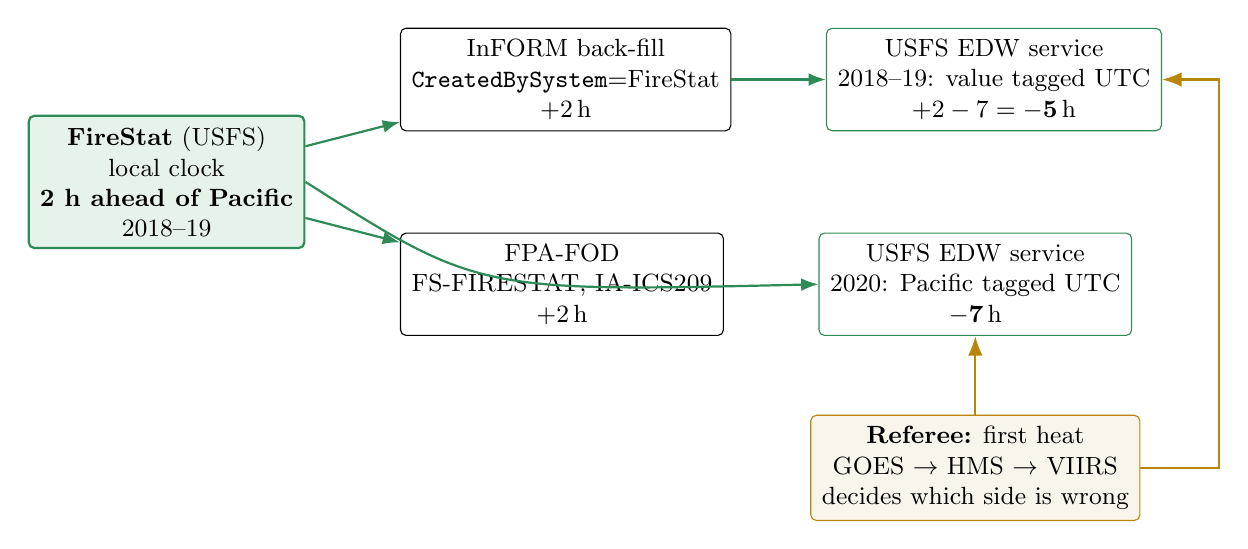
\begin{tikzpicture}[node distance=8mm and 12mm]
  \node[src, draw=usfs, thick, fill=palegreen] (fs) {\textbf{FireStat} (USFS)\\local clock\\\textbf{2 h ahead of Pacific}\\2018--19};
  \node[src, right=of fs, yshift=13mm] (inf) {InFORM back-fill\\\texttt{CreatedBySystem}=FireStat\\$+2$\,h};
  \node[src, right=of fs, yshift=-13mm] (fpa) {FPA-FOD\\FS-FIRESTAT, IA-ICS209\\$+2$\,h};
  \node[src, right=of inf, draw=usfs] (edw1) {USFS EDW service\\2018--19: value tagged UTC\\$+2 - 7 = \mathbf{-5}$\,h};
  \node[src, right=of fpa, draw=usfs] (edw2) {USFS EDW service\\2020: Pacific tagged UTC\\$\mathbf{-7}$\,h};
  \node[src, below=of edw2, draw=sat, fill=sat!8, yshift=-2mm] (ref) {\textbf{Referee:} first heat\\GOES $\to$ HMS $\to$ VIIRS\\decides which side is wrong};
  \draw[copy, usfs] (fs) -- (inf);
  \draw[copy, usfs] (fs) -- (fpa);
  \draw[copy, usfs] (inf) -- (edw1);
  \draw[copy, usfs] (fs.east) .. controls +(22mm,-14mm) .. (edw2.west);
  \draw[flow, sat] (ref) -- (edw2);
  \draw[flow, sat] (ref.east) -- ++(10mm,0) |- (edw1.east);
\end{tikzpicture}
\end{fitfig}
\caption{How one clock error appears as three different offsets. FireStat's 2018--19 times run two hours fast
(Delta 2018: FireStat 14:51 against 12:51 PDT in CAL~FIRE and IRWIN); the copies in InFORM and FPA-FOD inherit
$+2$\,h; the EDW map service labels FireStat's local value as UTC, which shows as $-5$\,h in 2018--19 (Delta is
served as 19:51Z) and $-7$\,h in 2020. 67 EDW records from 2018--2020 carry the error; EDW records from 2023 on
agree with IRWIN. The original catalog looked only for 7- and 8-hour offsets.}
\label{fig:clock}
\end{figure}

Because a whole-hour offset is symmetric, the audit cannot tell from two clocks alone which one is wrong. The
satellite referee resolves it: of the records at suspicious offsets, 67 USFS EDW records are flagged as the
erroneous side (2018: 20, 2019: 11, 2020: 36) and none are cleared, whereas 56 of 64 WFIGS records at such
offsets are cleared because the satellite sides with IRWIN. CAL~FIRE's incident list carries 26 whole-hour
errors of its own, 11 of them in 2020. FireSET inherits four.

%======================================================================
\section{Size and cause}

Reported final sizes agree with the consensus perimeter area to within 0.1\% at the median, because they are
mostly the same polygon's acreage. 114 fires nevertheless have at least one source more than 25\% off. The main
cause is IRWIN incident sizes never updated past discovery: 36 fires whose WFIGS \texttt{IncidentSize} is
0.01--0.3 acres against hundreds or thousands of acres mapped, an error that InFORM and FPA-FOD inherit. A
second cause was a field choice: WFIGS perimeters' \texttt{poly\_GISAcres} is a placeholder (0.1, 1 or 20 acres)
on many 2020 polygons, so the run uses \texttt{poly\_Acres\_AutoCalc}. MTBS's burned area is a median 1--2\%
larger than the agency figure.

Cause is reported by two or more sources for 570 fires and conflicts between human and natural on only three.
The consensus is Undetermined for 279 fires, Natural for 179 and Human for 128; the large Undetermined share is
genuine (IRWIN and FRAP both record ``undetermined'' or code 14), not a classification failure.

%======================================================================
\section{Insights}

\begin{enumerate}[leftmargin=*, itemsep=3pt]
\item \textbf{There is one upstream record, not many sources.} IRWIN is the system of record for wildfire
incidents since 2020, and WFIGS, InFORM, FPA-FOD and MTBS re-publish it. Counting them as corroboration
inflates confidence without adding information. FireSET's choice of WFIGS is the right one, but it means FireSET
cannot be confirmed by the ``federal'' sources at all; only CAL~FIRE's operational record, pre-2020 FireStat and
state reports, and the satellites are independent.
\item \textbf{A map pin is not a point of origin.} About a quarter of agency ignition points lie more than
375\,m outside the final perimeter. IRWIN's first-report location moves by more than 500\,m on 40\% of fires
before it settles. The honest precision of an ``ignition point'' in these systems is hundreds of metres, and
for a minority, kilometres.
\item \textbf{Timing is the strongest-confirmed attribute.} GOES-R puts first heat within an hour of FireSET's
start time on 70\% of fires it sees; IRWIN, CAL~FIRE and the state records agree with each other to the
minute. The errors that do exist are systematic clock errors in one system (FireStat), not noise, and can be
corrected by rule.
\item \textbf{Perimeter and size are a single measurement.} FRAP's polygon is \emph{the} polygon; the other
agency layers copy it and its acreage. MTBS is the one check, and it agrees to IoU 0.94 while being slightly
larger.
\item \textbf{Validating a dataset against live services is not the same as reading their metadata.} Seven
field-level defects (\S\ref{sec:catalog}) survived a metadata check. Each would have produced a confident,
wrong conclusion about FireSET.
\end{enumerate}

%======================================================================
\section{Recommendations for FireSET}

\begin{enumerate}[leftmargin=*, itemsep=3pt]
\item Apply the 62 \emph{replace} rows of \texttt{fireset\_ignition\_patch.csv} after a spot check of the 31 that
rest on a CAL~FIRE pin alone; keep the provenance column so each coordinate traces to an agency record.
\item Review the 65 \emph{review} rows in QGIS. The layers are \texttt{ignition\_points},
\texttt{consensus\_perimeters} and \texttt{source\_perimeters}; most rows are two plausible points inside one
perimeter.
\item Record an \emph{ignition precision} field: the number of decimals carried, whether the point lies inside the
final perimeter, and whether a second independent lineage exists. For 195 fires no second lineage exists.
\item Keep \texttt{Start\_Local}; it is confirmed by GOES-R. Where a USFS source is used for timing, correct the
2018--20 FireStat/EDW offsets by rule rather than by hand.
\item Treat FRAP and MTBS as the two perimeter measurements; ignore WFIGS/EDW/NIFC perimeters as duplicates.
\end{enumerate}

%======================================================================
\section{Limits of this audit}

\begin{itemize}[leftmargin=*, itemsep=2pt]
\item The GOES search is centred on FireSET's own point (5\,km radius), so it confirms timing but is not an
independent \emph{location} check. FireSET's own VIIRS \texttt{.h5} files were not available; the FIRMS S-NPP and
NOAA-20 yearly archives were used instead (no NOAA-21), with ``type 0'' detections only.
\item The recommended point is always an existing agency record scored on support, perimeter, satellite
proximity, trust and precision; the audit never synthesises coordinates except as a low-confidence VIIRS
fallback for fires with no agency point.
\item NASA FEDS perimeters, InciWeb and NIROPS infrared perimeters were not used (no archive endpoint, or manual
sources); the CAL~FIRE FIRIS view holds only the current season.
\item Thresholds (500\,m / 2\,km agreement, 375\,m perimeter tolerance, 12\,h lead window, IoU 0.7) are settings
in \texttt{settings.yaml}, not truths.
\end{itemize}

\appendix
\section{Reproducing the run}

{\small
\begin{verbatim}
git clone https://github.com/utkrshkmr/fire-data-revalid
cd fire-data-revalid
scripts/download_local_sources.sh          # FPA-FOD, MTBS, USGS, FIRMS (~2.5 GB)
cd fire-source-audit
python -m venv .venv && .venv/bin/pip install -e ".[dev,goes]"
cp /path/to/SUBSET_expanded_20260830.xlsx data/
.venv/bin/pytest -q                        # 24 tests
.venv/bin/fsa probe                        # every endpoint and field mapping
.venv/bin/fsa fetch --workers 6            # network sources -> cache/
.venv/bin/fsa --only viirs_firms_csv,hms_points fetch
.venv/bin/fsa --only goes_fdc fetch        # optional, ~20 min on 16 cores
.venv/bin/fsa analyze                      # -> out/
python ../scripts/summarize_findings.py out   # the numbers in this document
\end{verbatim}}

\section{Output files}

\begin{table}[h]
\centering\footnotesize
\begin{tabularx}{\textwidth}{@{}lY@{}}
\toprule
File & Contents\\
\midrule
\texttt{fire\_summary.csv} & one row per fire: consensus, agreement class, recommendation, satellite bounds, flags\\
\texttt{source\_errors.csv} & one row per fire $\times$ source $\times$ aspect, with every metric\\
\texttt{source\_summary.csv} & per-source statistics\\
\texttt{timing\_by\_lineage.csv} & discovery offsets per source and record lineage\\
\texttt{identical\_point\_pairs.csv} & every detected copy of a point between sources, by lineage\\
\texttt{perimeter\_pairs.csv} & IoU, area ratio and Hausdorff distance for every pair of perimeters\\
\texttt{flags.csv} & every issue, with category and severity\\
\texttt{fireset\_ignition\_patch.csv} & the 127 proposed corrections with action, evidence and provenance\\
\texttt{matched\_records.csv} & the crosswalk: which record in each source matched each fire, and how\\
\texttt{ignition\_points.geojson} & reported, consensus, recommended and first-VIIRS points per fire\\
\texttt{consensus\_perimeters.geojson}, \texttt{source\_perimeters.geojson} & perimeter layers for QGIS\\
\texttt{report.html}, \texttt{fire\_source\_audit.xlsx} & HTML summary with charts; the main tables in one workbook\\
\bottomrule
\end{tabularx}
\end{table}

\end{document}
